% Ejemplo de documento LaTeX
% Tipo de documento y tamaño de letra
\documentclass[12pt]{article}


\usepackage[spanish]{babel}
\usepackage{longtable} 
\selectlanguage{spanish}
\usepackage[utf8]{inputenc}
\usepackage{graphicx}




% EL titulo, autor y fecha del documento
\title{Reporte de Actividad 3}
\author{Carlos Medina}
\date{20-2-15}


% Aqui comienza el cuerpo del documento
\begin{document}
% Construye el título
\maketitle


El siguiente reporte describirá los pasos realizados para la actividad 3 (2015-1), así como ilustrará los resultados de ésta.




\hspace {0.5cm} Fortran 90 (previamente FORTRAN) es un lenguaje de programación alto nivel de propósito general, procedimenta e imperativo, que está especialmente adaptado al cálculo numérico y a la computación científica. Es el sucesor de FORTRAN 77, informalmente conocido como Fortran 90 (y anterior a eso, Fortran 8X), fue finalmente lanzado como ISO/IEC estándar en 1991 y un ANSI estándar en 1992. En adición de cambiar el nombre oficial de FORTRAN a Fortran,además de agregar muchas características nuevas para reflejar los cambios significativos en la práctica de la programación que ha evolucionado desde el estándar de 1978.




\hspace {0.5cm} A continuación veremos unos cálculos que se resolverán utilizando Fortran 90, de calcular áreas a funciones.
\vspace {0.5cm}
     Primero empezaremos calculando el área de un círculoe en función del radio que tú elijas:
     
     \begin{verbatim}
     
     Program circle_area
  Implicit None
  Real *8 :: radius, circum, area
  Real *8 :: PI = 4.0 * atan(1.0)
  Integer :: model_n = 1
  print *, 'enter a radius:'
  read (*,*) radius
  circum = 2.0 * PI * radius
  area = radius * radius * PI 
  print *, 'Program number =' , model_n
  print *, 'radius =' , radius
  print *, 'circumference =' , circum
  print *, 'area =' , area
end Program circle_area 
 
    
     \end{verbatim}
     
Después de compilar, procedemos a ejecutar el programa y escrubir el radio que deseamos, entonces nos saldrá la siguiente pantalla:
     
     

\begin{figure*}[h]
\hspace{-3.7cm}
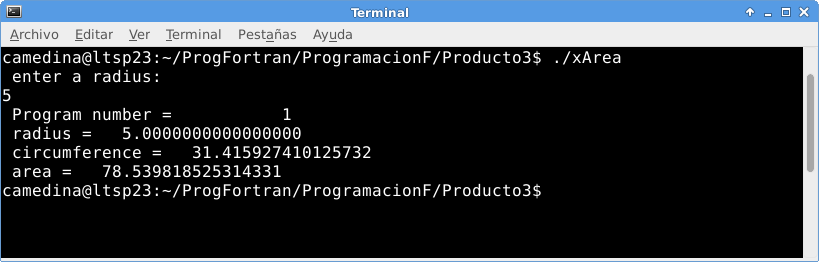
\includegraphics{1.png}{10pt}

\end{figure*}

 
 
% Nunca debe faltar esta última linea.
\end{document}